\documentclass[twoside]{book}

% Packages required by doxygen
\usepackage{calc}
\usepackage{doxygen}
\usepackage{graphicx}
\usepackage[utf8]{inputenc}
\usepackage{makeidx}
\usepackage{multicol}
\usepackage{multirow}
\usepackage{textcomp}
\usepackage[table]{xcolor}

% Font selection
\usepackage[T1]{fontenc}
\usepackage{mathptmx}
\usepackage[scaled=.90]{helvet}
\usepackage{courier}
\usepackage{amssymb}
\usepackage{sectsty}
\renewcommand{\familydefault}{\sfdefault}
\allsectionsfont{%
  \fontseries{bc}\selectfont%
  \color{darkgray}%
}
\renewcommand{\DoxyLabelFont}{%
  \fontseries{bc}\selectfont%
  \color{darkgray}%
}

% Page & text layout
\usepackage{geometry}
\geometry{%
  a4paper,%
  top=2.5cm,%
  bottom=2.5cm,%
  left=2.5cm,%
  right=2.5cm%
}
\tolerance=750
\hfuzz=15pt
\hbadness=750
\setlength{\emergencystretch}{15pt}
\setlength{\parindent}{0cm}
\setlength{\parskip}{0.2cm}
\makeatletter
\renewcommand{\paragraph}{%
  \@startsection{paragraph}{4}{0ex}{-1.0ex}{1.0ex}{%
    \normalfont\normalsize\bfseries\SS@parafont%
  }%
}
\renewcommand{\subparagraph}{%
  \@startsection{subparagraph}{5}{0ex}{-1.0ex}{1.0ex}{%
    \normalfont\normalsize\bfseries\SS@subparafont%
  }%
}
\makeatother

% Headers & footers
\usepackage{fancyhdr}
\pagestyle{fancyplain}
\fancyhead[LE]{\fancyplain{}{\bfseries\thepage}}
\fancyhead[CE]{\fancyplain{}{}}
\fancyhead[RE]{\fancyplain{}{\bfseries\leftmark}}
\fancyhead[LO]{\fancyplain{}{\bfseries\rightmark}}
\fancyhead[CO]{\fancyplain{}{}}
\fancyhead[RO]{\fancyplain{}{\bfseries\thepage}}
\fancyfoot[LE]{\fancyplain{}{}}
\fancyfoot[CE]{\fancyplain{}{}}
\fancyfoot[RE]{\fancyplain{}{\bfseries\scriptsize Generated on Sun Nov 15 2015 19\-:53\-:14 for Square Master-\/\-Blasters by Doxygen }}
\fancyfoot[LO]{\fancyplain{}{\bfseries\scriptsize Generated on Sun Nov 15 2015 19\-:53\-:14 for Square Master-\/\-Blasters by Doxygen }}
\fancyfoot[CO]{\fancyplain{}{}}
\fancyfoot[RO]{\fancyplain{}{}}
\renewcommand{\footrulewidth}{0.4pt}
\renewcommand{\chaptermark}[1]{%
  \markboth{#1}{}%
}
\renewcommand{\sectionmark}[1]{%
  \markright{\thesection\ #1}%
}

% Indices & bibliography
\usepackage{natbib}
\usepackage[titles]{tocloft}
\setcounter{tocdepth}{3}
\setcounter{secnumdepth}{5}
\makeindex

% Hyperlinks (required, but should be loaded last)
\usepackage{ifpdf}
\ifpdf
  \usepackage[pdftex,pagebackref=true]{hyperref}
\else
  \usepackage[ps2pdf,pagebackref=true]{hyperref}
\fi
\hypersetup{%
  colorlinks=true,%
  linkcolor=blue,%
  citecolor=blue,%
  unicode%
}

% Custom commands
\newcommand{\clearemptydoublepage}{%
  \newpage{\pagestyle{empty}\cleardoublepage}%
}


%===== C O N T E N T S =====

\begin{document}

% Titlepage & ToC
\hypersetup{pageanchor=false}
\pagenumbering{roman}
\begin{titlepage}
\vspace*{7cm}
\begin{center}%
{\Large Square Master-\/\-Blasters }\\
\vspace*{1cm}
{\large Generated by Doxygen 1.8.6}\\
\vspace*{0.5cm}
{\small Sun Nov 15 2015 19:53:14}\\
\end{center}
\end{titlepage}
\clearemptydoublepage
\tableofcontents
\clearemptydoublepage
\pagenumbering{arabic}
\hypersetup{pageanchor=true}

%--- Begin generated contents ---
\chapter{S\-E\-N\-G330}
\label{md_README}
\hypertarget{md_README}{}
S\-E\-N\-G 330 Group 10 Project Repository. Turn-\/based 2-\/player game -\/ name to be chosen.

\subsection*{Setup\-: }

We will be using Python 2.\-7, and Py\-Game. Follow download/setup instructions at \href{http://www.pygame.org/hifi.html}{\tt http\-://www.\-pygame.\-org/hifi.\-html}.

I have personally chosen to develop on Linux, and use virtualenv to create an isolated environment for this specific project. You can read about virtualenv here\-: \href{http://docs.python-guide.org/en/latest/dev/virtualenvs/}{\tt http\-://docs.\-python-\/guide.\-org/en/latest/dev/virtualenvs/}. But virtualenv is not necessary, and the project should work on Mac Windows or Linux.

Once you have cloned this project and have Py\-Game installed, try running game.\-py with the Python 2.\-7 interpreter.

-\/\-Will

\subsection*{Instructions\-: }

To move a character, select it on the grid with the mouse, press m on the keyboard, and select the square where you would like to move the character. 
\chapter{Hierarchical Index}
\section{Class Hierarchy}
This inheritance list is sorted roughly, but not completely, alphabetically\-:\begin{DoxyCompactList}
\item \contentsline{section}{game.\-Game}{\pageref{classgame_1_1Game}}{}
\item \contentsline{section}{game.\-Grid}{\pageref{classgame_1_1Grid}}{}
\item object\begin{DoxyCompactList}
\item \contentsline{section}{game.\-Grid\-Tile}{\pageref{classgame_1_1GridTile}}{}
\begin{DoxyCompactList}
\item \contentsline{section}{game.\-Character}{\pageref{classgame_1_1Character}}{}
\begin{DoxyCompactList}
\item \contentsline{section}{game.\-Bridget}{\pageref{classgame_1_1Bridget}}{}
\item \contentsline{section}{game.\-Doge}{\pageref{classgame_1_1Doge}}{}
\item \contentsline{section}{game.\-James}{\pageref{classgame_1_1James}}{}
\item \contentsline{section}{game.\-Moad}{\pageref{classgame_1_1Moad}}{}
\item \contentsline{section}{game.\-Wilfred}{\pageref{classgame_1_1Wilfred}}{}
\end{DoxyCompactList}
\end{DoxyCompactList}
\end{DoxyCompactList}
\item \contentsline{section}{game.\-Player}{\pageref{classgame_1_1Player}}{}
\end{DoxyCompactList}

\chapter{Class Index}
\section{Class List}
Here are the classes, structs, unions and interfaces with brief descriptions\-:\begin{DoxyCompactList}
\item\contentsline{section}{\hyperlink{classgame_1_1Bridget}{game.\-Bridget} }{\pageref{classgame_1_1Bridget}}{}
\item\contentsline{section}{\hyperlink{classgame_1_1Character}{game.\-Character} }{\pageref{classgame_1_1Character}}{}
\item\contentsline{section}{\hyperlink{classgame_1_1Doge}{game.\-Doge} }{\pageref{classgame_1_1Doge}}{}
\item\contentsline{section}{\hyperlink{classgame_1_1Game}{game.\-Game} }{\pageref{classgame_1_1Game}}{}
\item\contentsline{section}{\hyperlink{classgame_1_1Grid}{game.\-Grid} }{\pageref{classgame_1_1Grid}}{}
\item\contentsline{section}{\hyperlink{classgame_1_1GridTile}{game.\-Grid\-Tile} }{\pageref{classgame_1_1GridTile}}{}
\item\contentsline{section}{\hyperlink{classgame_1_1James}{game.\-James} }{\pageref{classgame_1_1James}}{}
\item\contentsline{section}{\hyperlink{classgame_1_1Moad}{game.\-Moad} }{\pageref{classgame_1_1Moad}}{}
\item\contentsline{section}{\hyperlink{classgame_1_1Player}{game.\-Player} }{\pageref{classgame_1_1Player}}{}
\item\contentsline{section}{\hyperlink{classgame_1_1Wilfred}{game.\-Wilfred} }{\pageref{classgame_1_1Wilfred}}{}
\end{DoxyCompactList}

\chapter{Class Documentation}
\hypertarget{classgame_1_1Bridget}{\section{game.\-Bridget Class Reference}
\label{classgame_1_1Bridget}\index{game.\-Bridget@{game.\-Bridget}}
}
Inheritance diagram for game.\-Bridget\-:\begin{figure}[H]
\begin{center}
\leavevmode
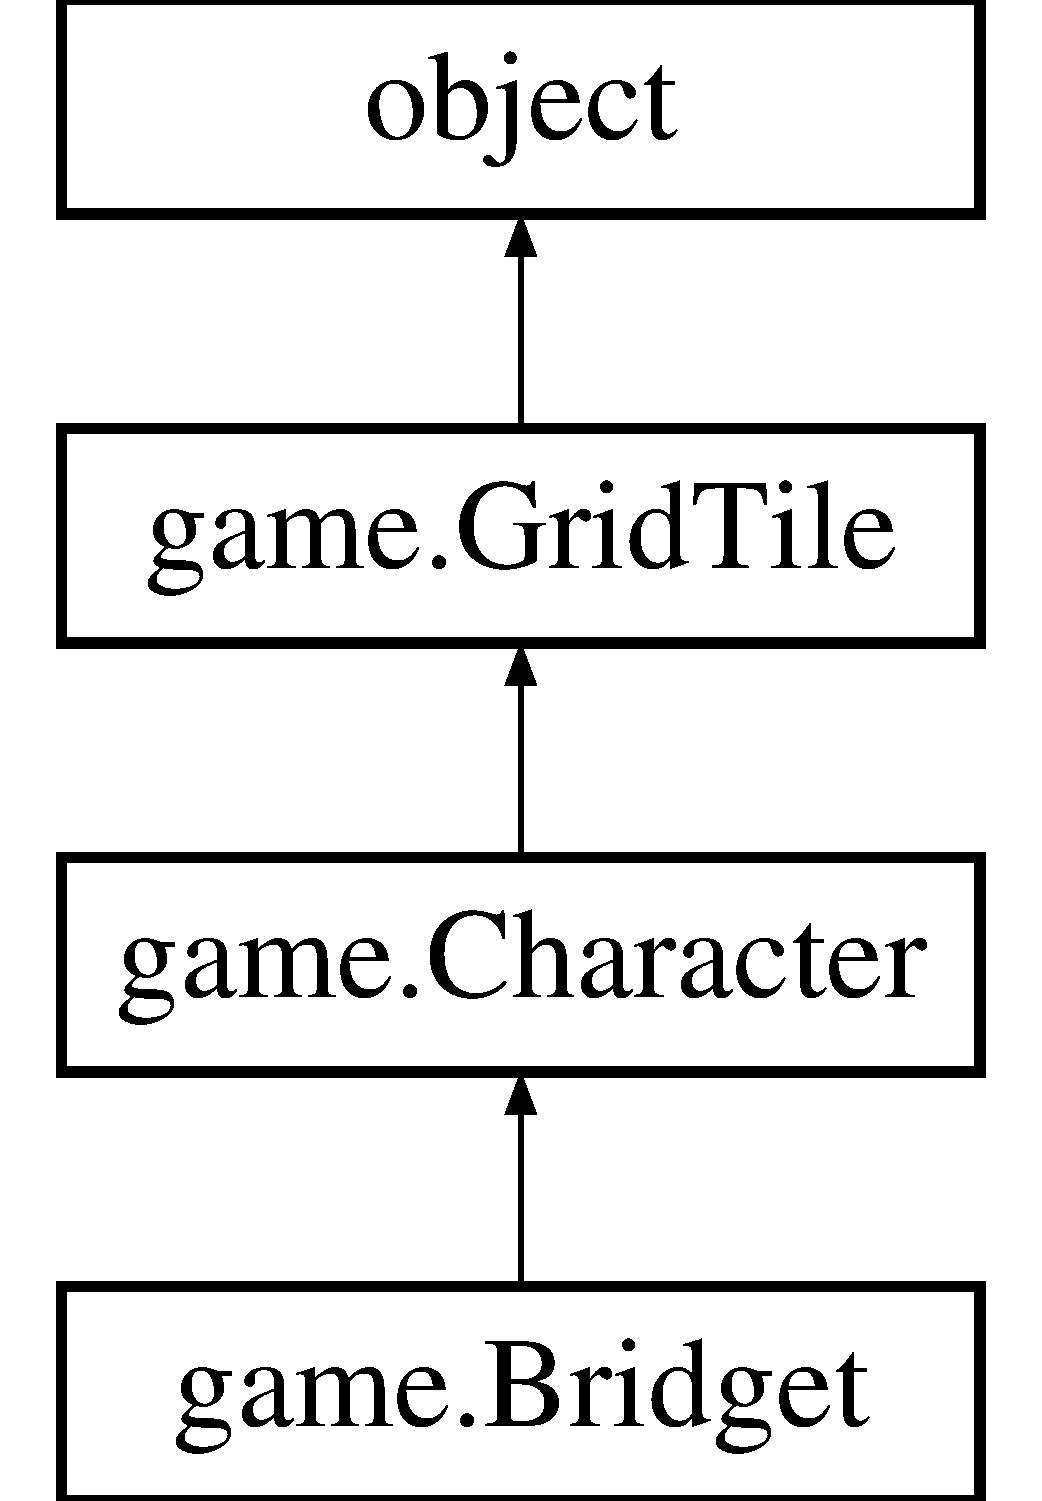
\includegraphics[height=4.000000cm]{classgame_1_1Bridget}
\end{center}
\end{figure}
\subsection*{Public Member Functions}
\begin{DoxyCompactItemize}
\item 
\hypertarget{classgame_1_1Bridget_ad4e6f9321bbaa2517223e7aedbf02506}{def {\bfseries \-\_\-\-\_\-init\-\_\-\-\_\-}}\label{classgame_1_1Bridget_ad4e6f9321bbaa2517223e7aedbf02506}

\end{DoxyCompactItemize}
\subsection*{Public Attributes}
\begin{DoxyCompactItemize}
\item 
\hypertarget{classgame_1_1Bridget_a31e484fbe78d55a092c758e90a089c06}{{\bfseries image}}\label{classgame_1_1Bridget_a31e484fbe78d55a092c758e90a089c06}

\item 
\hypertarget{classgame_1_1Bridget_a3db5aaacaad5161eccb76cc1f3d92f54}{{\bfseries move\-\_\-ability\-\_\-distance}}\label{classgame_1_1Bridget_a3db5aaacaad5161eccb76cc1f3d92f54}

\item 
\hypertarget{classgame_1_1Bridget_ae613de7294689a2ce89576205b6073e1}{{\bfseries attack\-\_\-ability\-\_\-distance}}\label{classgame_1_1Bridget_ae613de7294689a2ce89576205b6073e1}

\item 
\hypertarget{classgame_1_1Bridget_a2669cd98f86ef77b01e9f065ee1fce14}{{\bfseries attack\-\_\-power}}\label{classgame_1_1Bridget_a2669cd98f86ef77b01e9f065ee1fce14}

\item 
\hypertarget{classgame_1_1Bridget_adf25d85b6d474fa62352afaa85a60bf5}{{\bfseries health\-\_\-points}}\label{classgame_1_1Bridget_adf25d85b6d474fa62352afaa85a60bf5}

\end{DoxyCompactItemize}


The documentation for this class was generated from the following file\-:\begin{DoxyCompactItemize}
\item 
game.\-py\end{DoxyCompactItemize}

\hypertarget{classgame_1_1Character}{\section{game.\-Character Class Reference}
\label{classgame_1_1Character}\index{game.\-Character@{game.\-Character}}
}
Inheritance diagram for game.\-Character\-:\begin{figure}[H]
\begin{center}
\leavevmode
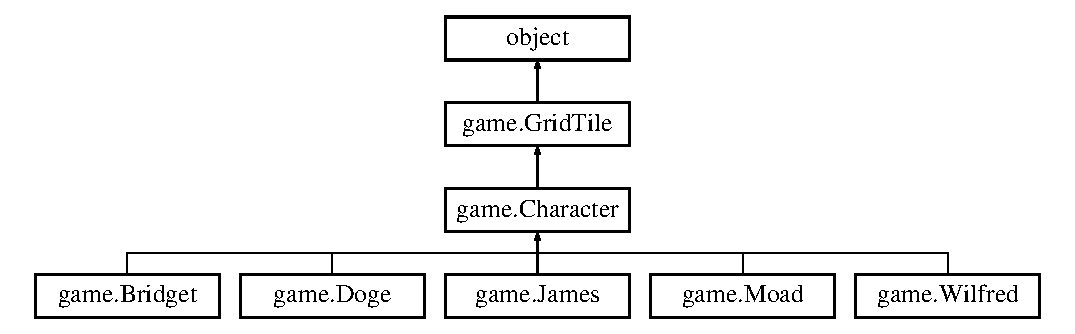
\includegraphics[height=4.000000cm]{classgame_1_1Character}
\end{center}
\end{figure}
\subsection*{Public Member Functions}
\begin{DoxyCompactItemize}
\item 
\hypertarget{classgame_1_1Character_a06269d574a3caba46fda1ab769bbe11a}{def {\bfseries \-\_\-\-\_\-init\-\_\-\-\_\-}}\label{classgame_1_1Character_a06269d574a3caba46fda1ab769bbe11a}

\item 
\hypertarget{classgame_1_1Character_ab4483704a8c8c8d0c3a2fe92caa13ad6}{def {\bfseries draw}}\label{classgame_1_1Character_ab4483704a8c8c8d0c3a2fe92caa13ad6}

\item 
\hypertarget{classgame_1_1Character_a377f9ea59ab4a461f15064d033577eb5}{def {\bfseries draw\-\_\-border}}\label{classgame_1_1Character_a377f9ea59ab4a461f15064d033577eb5}

\end{DoxyCompactItemize}
\subsection*{Public Attributes}
\begin{DoxyCompactItemize}
\item 
\hypertarget{classgame_1_1Character_a24edd8eba429b95871d2aba45a782ed8}{{\bfseries x}}\label{classgame_1_1Character_a24edd8eba429b95871d2aba45a782ed8}

\item 
\hypertarget{classgame_1_1Character_a69b149b26ed88cf5f7c0cb96dd84e8e8}{{\bfseries y}}\label{classgame_1_1Character_a69b149b26ed88cf5f7c0cb96dd84e8e8}

\item 
\hypertarget{classgame_1_1Character_a7c0f72230651ffbe370001fdc55c9e00}{{\bfseries selected}}\label{classgame_1_1Character_a7c0f72230651ffbe370001fdc55c9e00}

\item 
\hypertarget{classgame_1_1Character_a2c9932edc776eb9214bbf1a48398174e}{{\bfseries owner}}\label{classgame_1_1Character_a2c9932edc776eb9214bbf1a48398174e}

\item 
\hypertarget{classgame_1_1Character_ac3f9c3f85636513c19c7865f3a4e0622}{{\bfseries image}}\label{classgame_1_1Character_ac3f9c3f85636513c19c7865f3a4e0622}

\item 
\hypertarget{classgame_1_1Character_a1b4c8be47c49498885f6445bffe6c191}{{\bfseries move\-\_\-ability\-\_\-distance}}\label{classgame_1_1Character_a1b4c8be47c49498885f6445bffe6c191}

\item 
\hypertarget{classgame_1_1Character_aa63dfab6c6341366d7d22dc2bdc48b9f}{{\bfseries attack\-\_\-ability\-\_\-distance}}\label{classgame_1_1Character_aa63dfab6c6341366d7d22dc2bdc48b9f}

\item 
\hypertarget{classgame_1_1Character_a4e53fa5563ec68809d921c8ef91bbcc7}{{\bfseries attack\-\_\-power}}\label{classgame_1_1Character_a4e53fa5563ec68809d921c8ef91bbcc7}

\item 
\hypertarget{classgame_1_1Character_a3b145280dac0ad06df842ec28cd4c559}{{\bfseries health\-\_\-points}}\label{classgame_1_1Character_a3b145280dac0ad06df842ec28cd4c559}

\end{DoxyCompactItemize}


The documentation for this class was generated from the following file\-:\begin{DoxyCompactItemize}
\item 
game.\-py\end{DoxyCompactItemize}

\hypertarget{classgame_1_1Doge}{\section{game.\-Doge Class Reference}
\label{classgame_1_1Doge}\index{game.\-Doge@{game.\-Doge}}
}
Inheritance diagram for game.\-Doge\-:\begin{figure}[H]
\begin{center}
\leavevmode
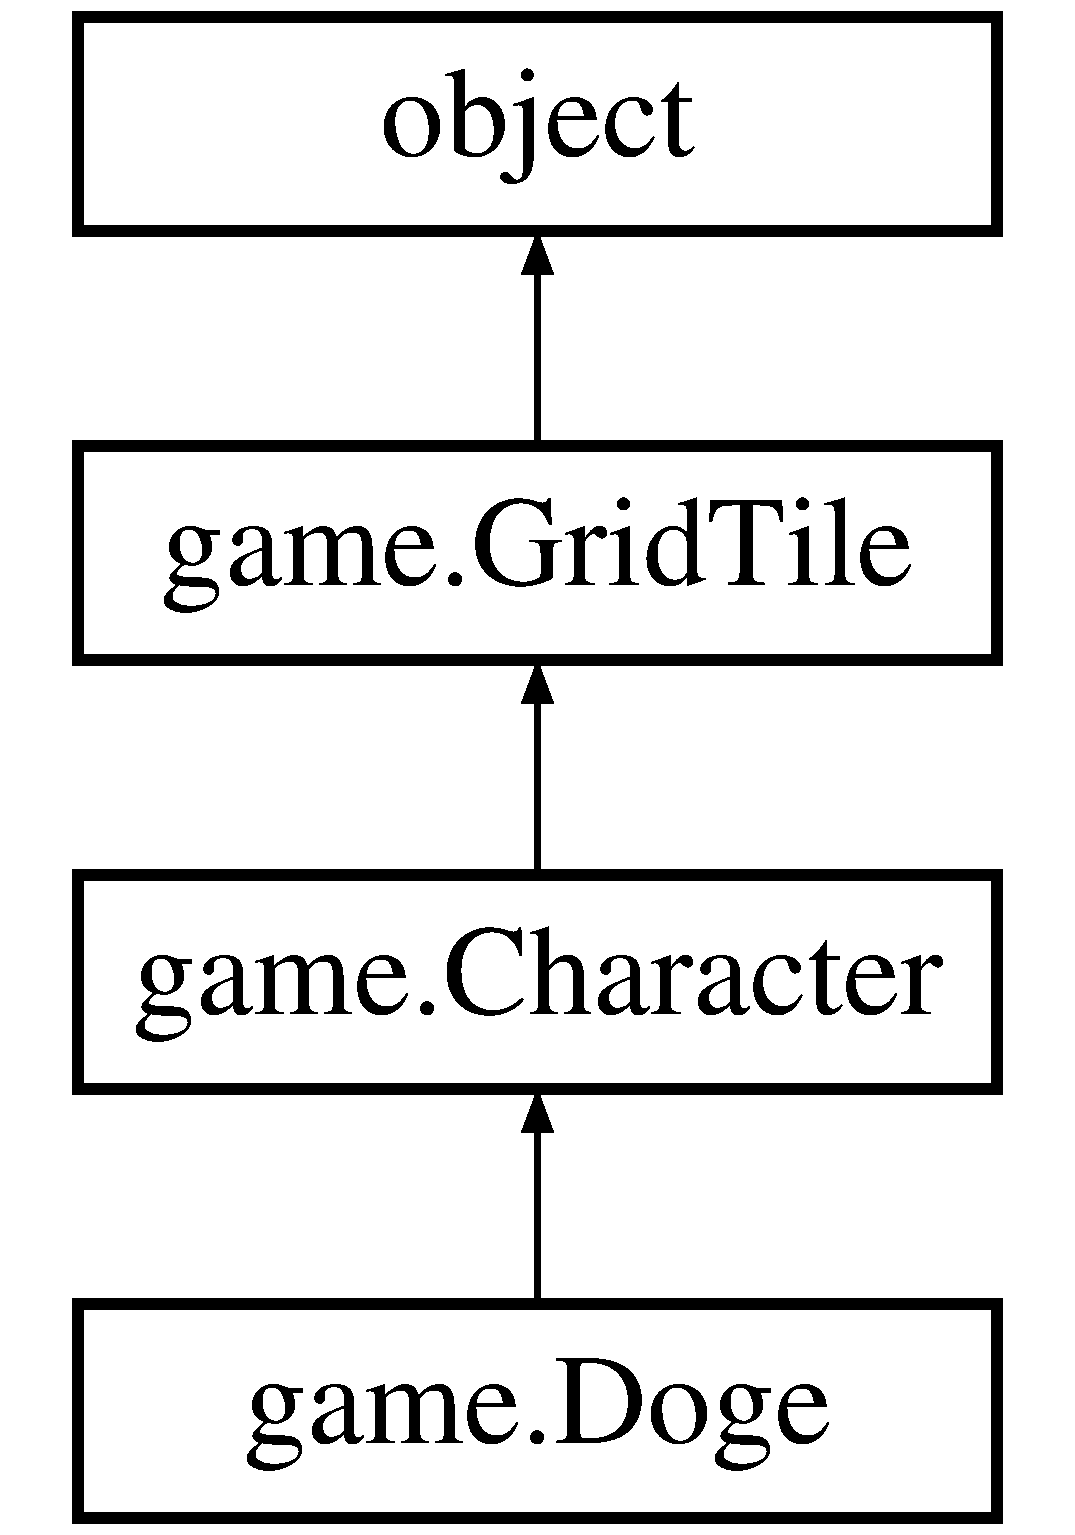
\includegraphics[height=4.000000cm]{classgame_1_1Doge}
\end{center}
\end{figure}
\subsection*{Public Member Functions}
\begin{DoxyCompactItemize}
\item 
\hypertarget{classgame_1_1Doge_ac666256c526db182cac3df5ab8279d58}{def {\bfseries \-\_\-\-\_\-init\-\_\-\-\_\-}}\label{classgame_1_1Doge_ac666256c526db182cac3df5ab8279d58}

\end{DoxyCompactItemize}
\subsection*{Public Attributes}
\begin{DoxyCompactItemize}
\item 
\hypertarget{classgame_1_1Doge_a38c30ac4cdc4a80041248a292b070262}{{\bfseries image}}\label{classgame_1_1Doge_a38c30ac4cdc4a80041248a292b070262}

\item 
\hypertarget{classgame_1_1Doge_a855030278537b5c912b93a5957269c8a}{{\bfseries move\-\_\-ability\-\_\-distance}}\label{classgame_1_1Doge_a855030278537b5c912b93a5957269c8a}

\item 
\hypertarget{classgame_1_1Doge_a8881ac6cb9a8f3309cf186fd46e1305d}{{\bfseries attack\-\_\-ability\-\_\-distance}}\label{classgame_1_1Doge_a8881ac6cb9a8f3309cf186fd46e1305d}

\item 
\hypertarget{classgame_1_1Doge_ad8fafec5441315fa4f65ced3c455836e}{{\bfseries attack\-\_\-power}}\label{classgame_1_1Doge_ad8fafec5441315fa4f65ced3c455836e}

\item 
\hypertarget{classgame_1_1Doge_a83a2d9ddb037115733b884050d225ec3}{{\bfseries health\-\_\-points}}\label{classgame_1_1Doge_a83a2d9ddb037115733b884050d225ec3}

\end{DoxyCompactItemize}


The documentation for this class was generated from the following file\-:\begin{DoxyCompactItemize}
\item 
game.\-py\end{DoxyCompactItemize}

\hypertarget{classgame_1_1Game}{\section{game.\-Game Class Reference}
\label{classgame_1_1Game}\index{game.\-Game@{game.\-Game}}
}
\subsection*{Public Member Functions}
\begin{DoxyCompactItemize}
\item 
\hypertarget{classgame_1_1Game_a8f52bb5e9eb9b75037d03347e21be0c5}{def {\bfseries \-\_\-\-\_\-init\-\_\-\-\_\-}}\label{classgame_1_1Game_a8f52bb5e9eb9b75037d03347e21be0c5}

\item 
\hypertarget{classgame_1_1Game_a57dd6c67fa5932339f29c67a7b20c2e4}{def {\bfseries display\-\_\-turn\-\_\-status}}\label{classgame_1_1Game_a57dd6c67fa5932339f29c67a7b20c2e4}

\item 
\hypertarget{classgame_1_1Game_ad6242e522d0dd0c4ec2d211ddc3202a8}{def {\bfseries display\-\_\-instructions}}\label{classgame_1_1Game_ad6242e522d0dd0c4ec2d211ddc3202a8}

\item 
\hypertarget{classgame_1_1Game_a19f1db5c572b4e6388fa38dc3c45d596}{def {\bfseries run}}\label{classgame_1_1Game_a19f1db5c572b4e6388fa38dc3c45d596}

\end{DoxyCompactItemize}
\subsection*{Static Public Member Functions}
\begin{DoxyCompactItemize}
\item 
\hypertarget{classgame_1_1Game_af3d3ad5543afe057a3ff1d8056001922}{def {\bfseries text\-\_\-objects}}\label{classgame_1_1Game_af3d3ad5543afe057a3ff1d8056001922}

\end{DoxyCompactItemize}
\subsection*{Public Attributes}
\begin{DoxyCompactItemize}
\item 
\hypertarget{classgame_1_1Game_a7379d6f60c3dcd68c0edf0966c2d3697}{{\bfseries window\-Surface}}\label{classgame_1_1Game_a7379d6f60c3dcd68c0edf0966c2d3697}

\item 
\hypertarget{classgame_1_1Game_a52a8c922ba616a54f3b2c0579be1426d}{{\bfseries grid}}\label{classgame_1_1Game_a52a8c922ba616a54f3b2c0579be1426d}

\item 
\hypertarget{classgame_1_1Game_a7cbd49dcf3f748850547f453583934cf}{{\bfseries player1}}\label{classgame_1_1Game_a7cbd49dcf3f748850547f453583934cf}

\item 
\hypertarget{classgame_1_1Game_aee8634f00ac6fdb2e99cc4c5de8f79e6}{{\bfseries player2}}\label{classgame_1_1Game_aee8634f00ac6fdb2e99cc4c5de8f79e6}

\item 
\hypertarget{classgame_1_1Game_aec618842be48a9664204a012bec01321}{{\bfseries player\-\_\-turn}}\label{classgame_1_1Game_aec618842be48a9664204a012bec01321}

\end{DoxyCompactItemize}


The documentation for this class was generated from the following file\-:\begin{DoxyCompactItemize}
\item 
game.\-py\end{DoxyCompactItemize}

\hypertarget{classgame_1_1Grid}{\section{game.\-Grid Class Reference}
\label{classgame_1_1Grid}\index{game.\-Grid@{game.\-Grid}}
}
\subsection*{Public Member Functions}
\begin{DoxyCompactItemize}
\item 
\hypertarget{classgame_1_1Grid_acb70672526797a8800f5dfe90c2e31aa}{def {\bfseries \-\_\-\-\_\-init\-\_\-\-\_\-}}\label{classgame_1_1Grid_acb70672526797a8800f5dfe90c2e31aa}

\item 
\hypertarget{classgame_1_1Grid_a504aee27da6bc3d501b8df1feb4d9d5c}{def {\bfseries draw}}\label{classgame_1_1Grid_a504aee27da6bc3d501b8df1feb4d9d5c}

\item 
\hypertarget{classgame_1_1Grid_a27ebe0a3f3b8586ffeb8441778e52089}{def {\bfseries select\-\_\-tile}}\label{classgame_1_1Grid_a27ebe0a3f3b8586ffeb8441778e52089}

\end{DoxyCompactItemize}
\subsection*{Public Attributes}
\begin{DoxyCompactItemize}
\item 
\hypertarget{classgame_1_1Grid_a660850041b0d33a59e6674afc2e39d47}{{\bfseries grid}}\label{classgame_1_1Grid_a660850041b0d33a59e6674afc2e39d47}

\item 
\hypertarget{classgame_1_1Grid_a563c2421b9a4308e47953c1563b66b16}{{\bfseries current\-\_\-tile}}\label{classgame_1_1Grid_a563c2421b9a4308e47953c1563b66b16}

\end{DoxyCompactItemize}


The documentation for this class was generated from the following file\-:\begin{DoxyCompactItemize}
\item 
game.\-py\end{DoxyCompactItemize}

\hypertarget{classgame_1_1GridTile}{\section{game.\-Grid\-Tile Class Reference}
\label{classgame_1_1GridTile}\index{game.\-Grid\-Tile@{game.\-Grid\-Tile}}
}
Inheritance diagram for game.\-Grid\-Tile\-:\begin{figure}[H]
\begin{center}
\leavevmode
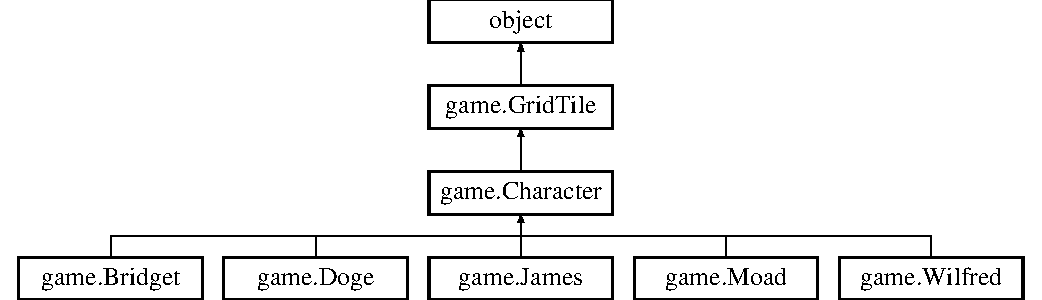
\includegraphics[height=4.000000cm]{classgame_1_1GridTile}
\end{center}
\end{figure}
\subsection*{Public Member Functions}
\begin{DoxyCompactItemize}
\item 
\hypertarget{classgame_1_1GridTile_a30ee8976e7630e986896d66bf3529cb1}{def {\bfseries \-\_\-\-\_\-init\-\_\-\-\_\-}}\label{classgame_1_1GridTile_a30ee8976e7630e986896d66bf3529cb1}

\item 
\hypertarget{classgame_1_1GridTile_a7dcddf78ff6e1130d140711c97529330}{def {\bfseries select}}\label{classgame_1_1GridTile_a7dcddf78ff6e1130d140711c97529330}

\item 
\hypertarget{classgame_1_1GridTile_ae2bc20ca4845608079fe3aa69630f820}{def {\bfseries deselect}}\label{classgame_1_1GridTile_ae2bc20ca4845608079fe3aa69630f820}

\item 
\hypertarget{classgame_1_1GridTile_afc0ebde63e213a9a4b930431cf60828c}{def {\bfseries set\-\_\-coordinates}}\label{classgame_1_1GridTile_afc0ebde63e213a9a4b930431cf60828c}

\item 
\hypertarget{classgame_1_1GridTile_a322a252e74a30c2466554d2a35d4144e}{def {\bfseries draw}}\label{classgame_1_1GridTile_a322a252e74a30c2466554d2a35d4144e}

\item 
\hypertarget{classgame_1_1GridTile_a77e0987e5c2539f3ad2964945dc29ed9}{def {\bfseries draw\-\_\-border}}\label{classgame_1_1GridTile_a77e0987e5c2539f3ad2964945dc29ed9}

\end{DoxyCompactItemize}
\subsection*{Public Attributes}
\begin{DoxyCompactItemize}
\item 
\hypertarget{classgame_1_1GridTile_aaf405723011f6d0b226713bf57fa9761}{{\bfseries x}}\label{classgame_1_1GridTile_aaf405723011f6d0b226713bf57fa9761}

\item 
\hypertarget{classgame_1_1GridTile_ae897d68c280cc0d0927f50093a036c00}{{\bfseries y}}\label{classgame_1_1GridTile_ae897d68c280cc0d0927f50093a036c00}

\item 
\hypertarget{classgame_1_1GridTile_afa378f455ed5696bee6f1baedb6f8e8e}{{\bfseries selected}}\label{classgame_1_1GridTile_afa378f455ed5696bee6f1baedb6f8e8e}

\end{DoxyCompactItemize}


The documentation for this class was generated from the following file\-:\begin{DoxyCompactItemize}
\item 
game.\-py\end{DoxyCompactItemize}

\hypertarget{classgame_1_1James}{\section{game.\-James Class Reference}
\label{classgame_1_1James}\index{game.\-James@{game.\-James}}
}
Inheritance diagram for game.\-James\-:\begin{figure}[H]
\begin{center}
\leavevmode
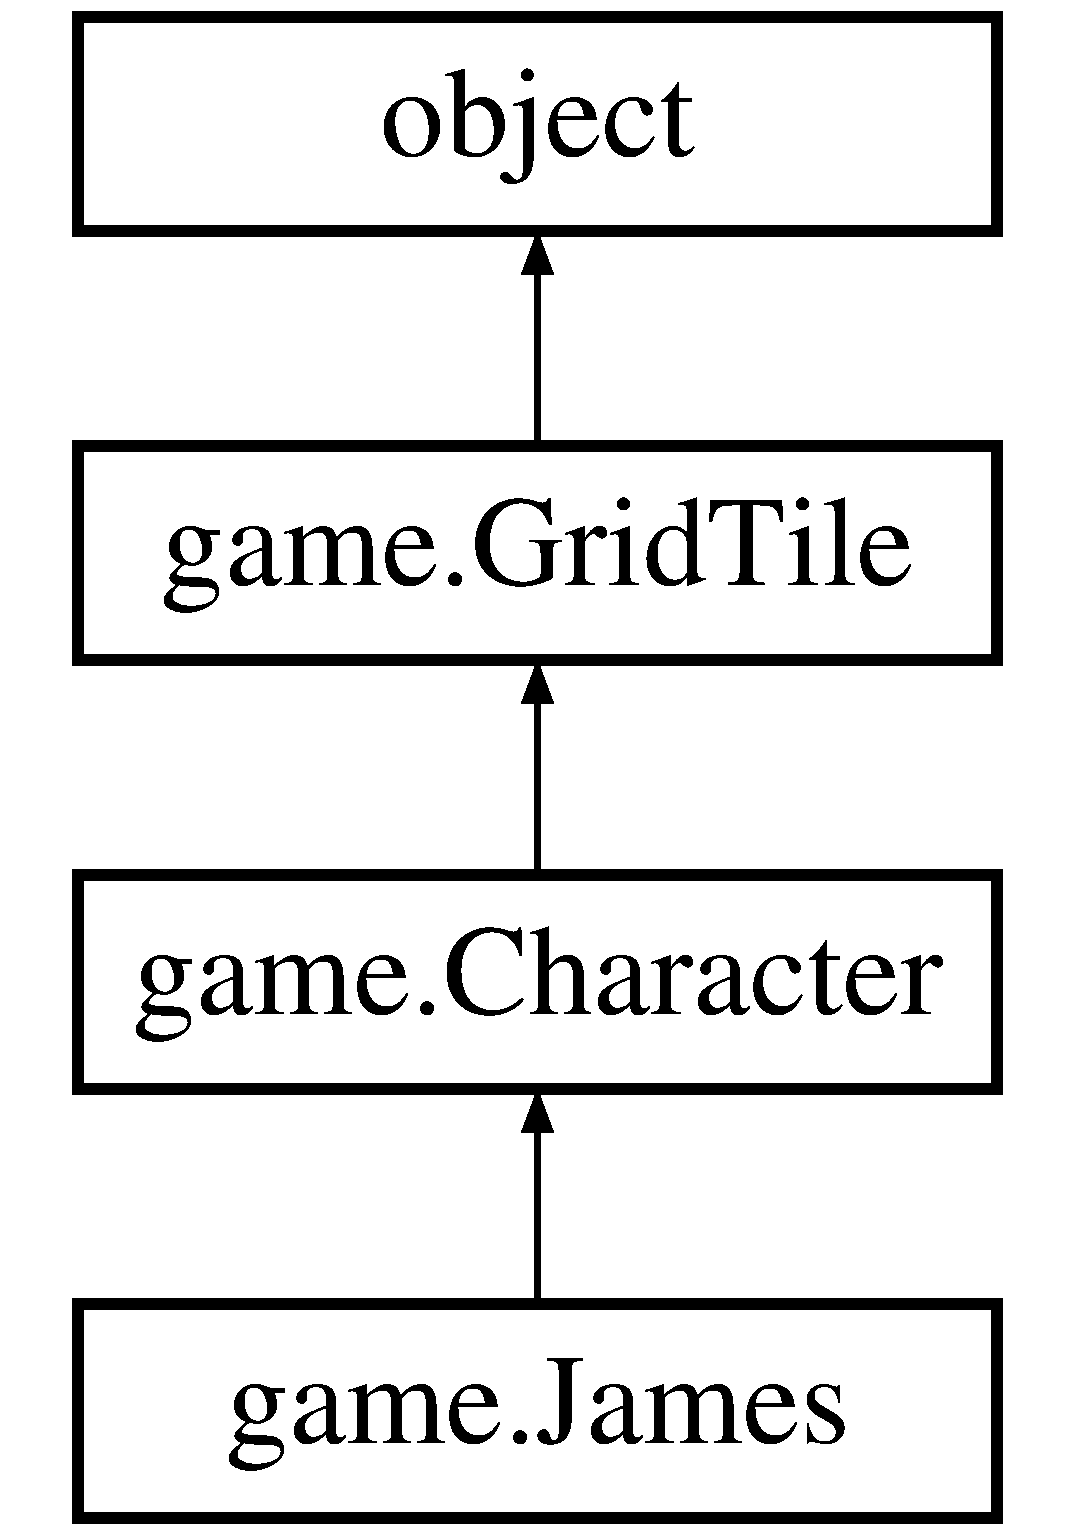
\includegraphics[height=4.000000cm]{classgame_1_1James}
\end{center}
\end{figure}
\subsection*{Public Member Functions}
\begin{DoxyCompactItemize}
\item 
\hypertarget{classgame_1_1James_ad5a69f9fa2b4826c3049aa64a10a9230}{def {\bfseries \-\_\-\-\_\-init\-\_\-\-\_\-}}\label{classgame_1_1James_ad5a69f9fa2b4826c3049aa64a10a9230}

\end{DoxyCompactItemize}
\subsection*{Public Attributes}
\begin{DoxyCompactItemize}
\item 
\hypertarget{classgame_1_1James_a80d7a25b9e092b647d15210a350159af}{{\bfseries image}}\label{classgame_1_1James_a80d7a25b9e092b647d15210a350159af}

\item 
\hypertarget{classgame_1_1James_a5bf9fd83a693a20a1d15286a36586b22}{{\bfseries move\-\_\-ability\-\_\-distance}}\label{classgame_1_1James_a5bf9fd83a693a20a1d15286a36586b22}

\item 
\hypertarget{classgame_1_1James_a5412e38e60f9385daddcb66d9d9cc851}{{\bfseries attack\-\_\-ability\-\_\-distance}}\label{classgame_1_1James_a5412e38e60f9385daddcb66d9d9cc851}

\item 
\hypertarget{classgame_1_1James_ae85fc663dbfc04f0ad0ca22d74ef96a8}{{\bfseries attack\-\_\-power}}\label{classgame_1_1James_ae85fc663dbfc04f0ad0ca22d74ef96a8}

\item 
\hypertarget{classgame_1_1James_a3dbfe488804ef3cbd605813a0030e89a}{{\bfseries health\-\_\-points}}\label{classgame_1_1James_a3dbfe488804ef3cbd605813a0030e89a}

\end{DoxyCompactItemize}


The documentation for this class was generated from the following file\-:\begin{DoxyCompactItemize}
\item 
game.\-py\end{DoxyCompactItemize}

\hypertarget{classgame_1_1Moad}{\section{game.\-Moad Class Reference}
\label{classgame_1_1Moad}\index{game.\-Moad@{game.\-Moad}}
}
Inheritance diagram for game.\-Moad\-:\begin{figure}[H]
\begin{center}
\leavevmode
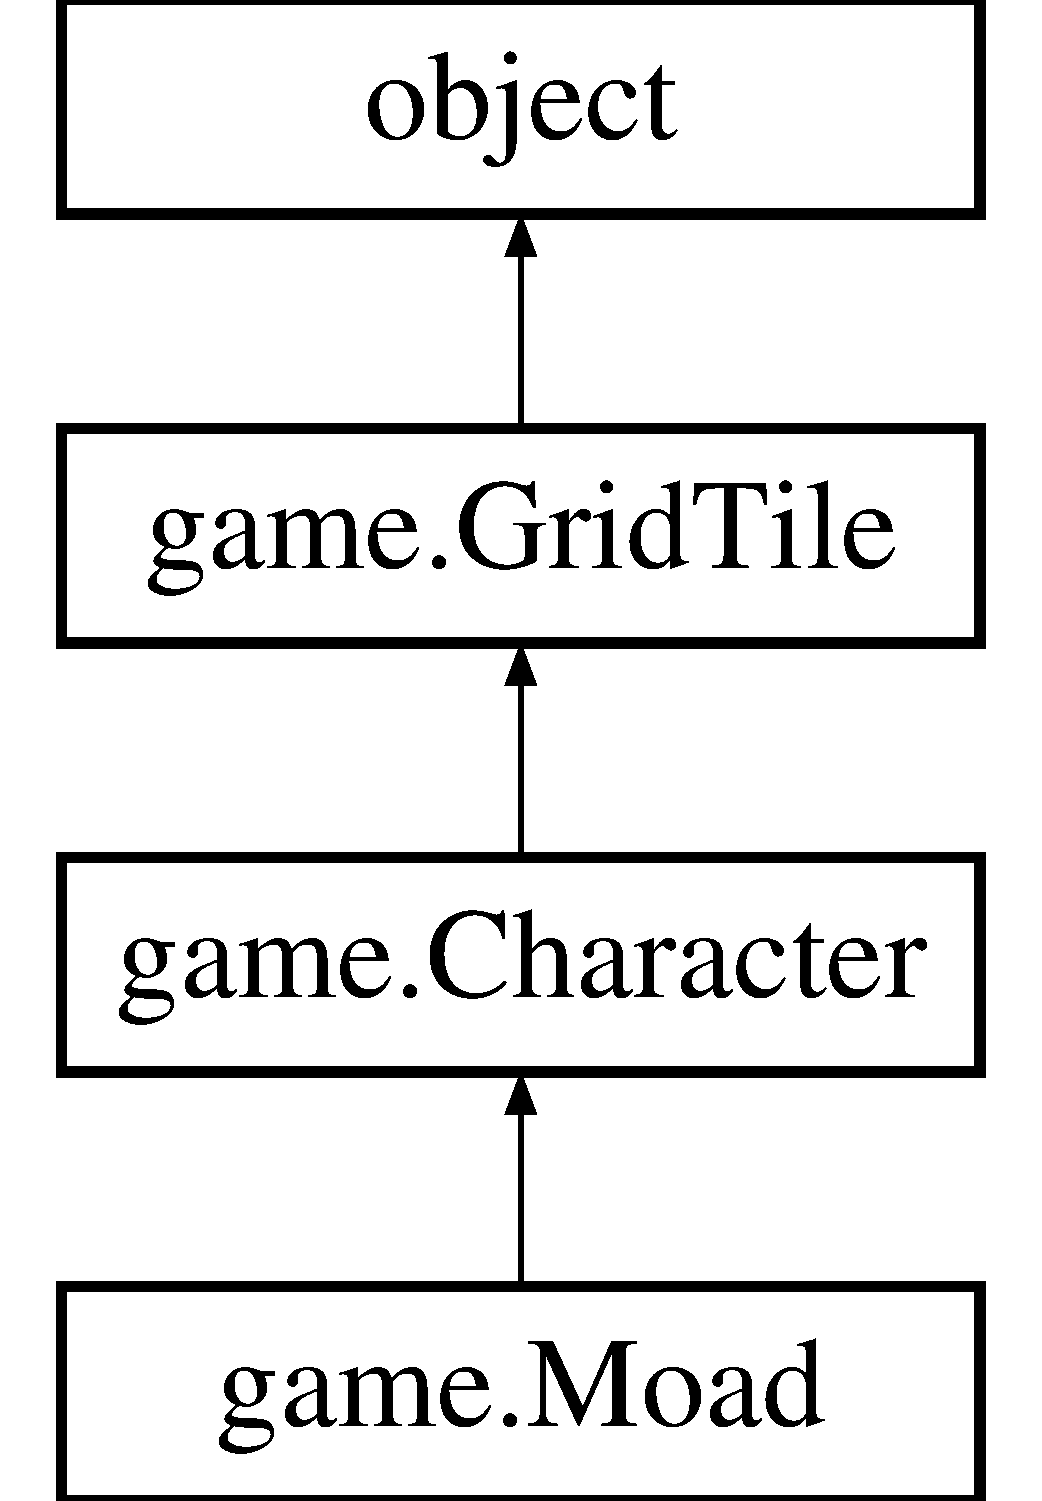
\includegraphics[height=4.000000cm]{classgame_1_1Moad}
\end{center}
\end{figure}
\subsection*{Public Member Functions}
\begin{DoxyCompactItemize}
\item 
\hypertarget{classgame_1_1Moad_aab657173104667983ded6c3918ecec3b}{def {\bfseries \-\_\-\-\_\-init\-\_\-\-\_\-}}\label{classgame_1_1Moad_aab657173104667983ded6c3918ecec3b}

\end{DoxyCompactItemize}
\subsection*{Public Attributes}
\begin{DoxyCompactItemize}
\item 
\hypertarget{classgame_1_1Moad_ad1133bb7dea5d6599b604320ff3844fa}{{\bfseries image}}\label{classgame_1_1Moad_ad1133bb7dea5d6599b604320ff3844fa}

\item 
\hypertarget{classgame_1_1Moad_a74e28dcf865aafe1cf6bb55368986028}{{\bfseries move\-\_\-ability\-\_\-distance}}\label{classgame_1_1Moad_a74e28dcf865aafe1cf6bb55368986028}

\item 
\hypertarget{classgame_1_1Moad_aec7bb1129561023ad5e08f621f89aba0}{{\bfseries attack\-\_\-ability\-\_\-distance}}\label{classgame_1_1Moad_aec7bb1129561023ad5e08f621f89aba0}

\item 
\hypertarget{classgame_1_1Moad_a176ec7ca641ea1e8f6d322c58dd1c3d2}{{\bfseries attack\-\_\-power}}\label{classgame_1_1Moad_a176ec7ca641ea1e8f6d322c58dd1c3d2}

\item 
\hypertarget{classgame_1_1Moad_a9cb430c08b2a176133d925850569ee70}{{\bfseries health\-\_\-points}}\label{classgame_1_1Moad_a9cb430c08b2a176133d925850569ee70}

\end{DoxyCompactItemize}


The documentation for this class was generated from the following file\-:\begin{DoxyCompactItemize}
\item 
game.\-py\end{DoxyCompactItemize}

\hypertarget{classgame_1_1Player}{\section{game.\-Player Class Reference}
\label{classgame_1_1Player}\index{game.\-Player@{game.\-Player}}
}
\subsection*{Public Member Functions}
\begin{DoxyCompactItemize}
\item 
\hypertarget{classgame_1_1Player_aac645b679755efbae936ff8a378227cc}{def {\bfseries \-\_\-\-\_\-init\-\_\-\-\_\-}}\label{classgame_1_1Player_aac645b679755efbae936ff8a378227cc}

\item 
\hypertarget{classgame_1_1Player_acadb4c840f7364f7b3f7da16c209677f}{def {\bfseries add\-\_\-character}}\label{classgame_1_1Player_acadb4c840f7364f7b3f7da16c209677f}

\item 
\hypertarget{classgame_1_1Player_a62f144e05578deb655e8fd3cc9769b0e}{def {\bfseries remove\-\_\-character}}\label{classgame_1_1Player_a62f144e05578deb655e8fd3cc9769b0e}

\item 
\hypertarget{classgame_1_1Player_aea17a68c8e2d8d3ac7e5f02eca99310b}{def {\bfseries move\-\_\-character}}\label{classgame_1_1Player_aea17a68c8e2d8d3ac7e5f02eca99310b}

\item 
\hypertarget{classgame_1_1Player_adff1b583fa0f0956cc58dece9a76fb84}{def {\bfseries attack\-\_\-character}}\label{classgame_1_1Player_adff1b583fa0f0956cc58dece9a76fb84}

\item 
\hypertarget{classgame_1_1Player_a09b379bcd67b9545fffc50589b501b65}{def {\bfseries use\-\_\-action}}\label{classgame_1_1Player_a09b379bcd67b9545fffc50589b501b65}

\item 
\hypertarget{classgame_1_1Player_abcb0b1a8932098fdcd2571e91871d27d}{def {\bfseries restore\-\_\-actions}}\label{classgame_1_1Player_abcb0b1a8932098fdcd2571e91871d27d}

\item 
\hypertarget{classgame_1_1Player_a0a20f60b83f64909b12dc68a9afba7a9}{def {\bfseries has\-\_\-actions}}\label{classgame_1_1Player_a0a20f60b83f64909b12dc68a9afba7a9}

\end{DoxyCompactItemize}
\subsection*{Public Attributes}
\begin{DoxyCompactItemize}
\item 
\hypertarget{classgame_1_1Player_ae4dd0e9c778731b2e363ec4844c5fbb9}{{\bfseries board}}\label{classgame_1_1Player_ae4dd0e9c778731b2e363ec4844c5fbb9}

\item 
\hypertarget{classgame_1_1Player_aea7a1bfe861faf23a2eb464c5bd8702d}{{\bfseries characters}}\label{classgame_1_1Player_aea7a1bfe861faf23a2eb464c5bd8702d}

\item 
\hypertarget{classgame_1_1Player_a27305ff4a94da59fe209adb7e4917012}{{\bfseries actions}}\label{classgame_1_1Player_a27305ff4a94da59fe209adb7e4917012}

\end{DoxyCompactItemize}


The documentation for this class was generated from the following file\-:\begin{DoxyCompactItemize}
\item 
game.\-py\end{DoxyCompactItemize}

\hypertarget{classgame_1_1Wilfred}{\section{game.\-Wilfred Class Reference}
\label{classgame_1_1Wilfred}\index{game.\-Wilfred@{game.\-Wilfred}}
}
Inheritance diagram for game.\-Wilfred\-:\begin{figure}[H]
\begin{center}
\leavevmode
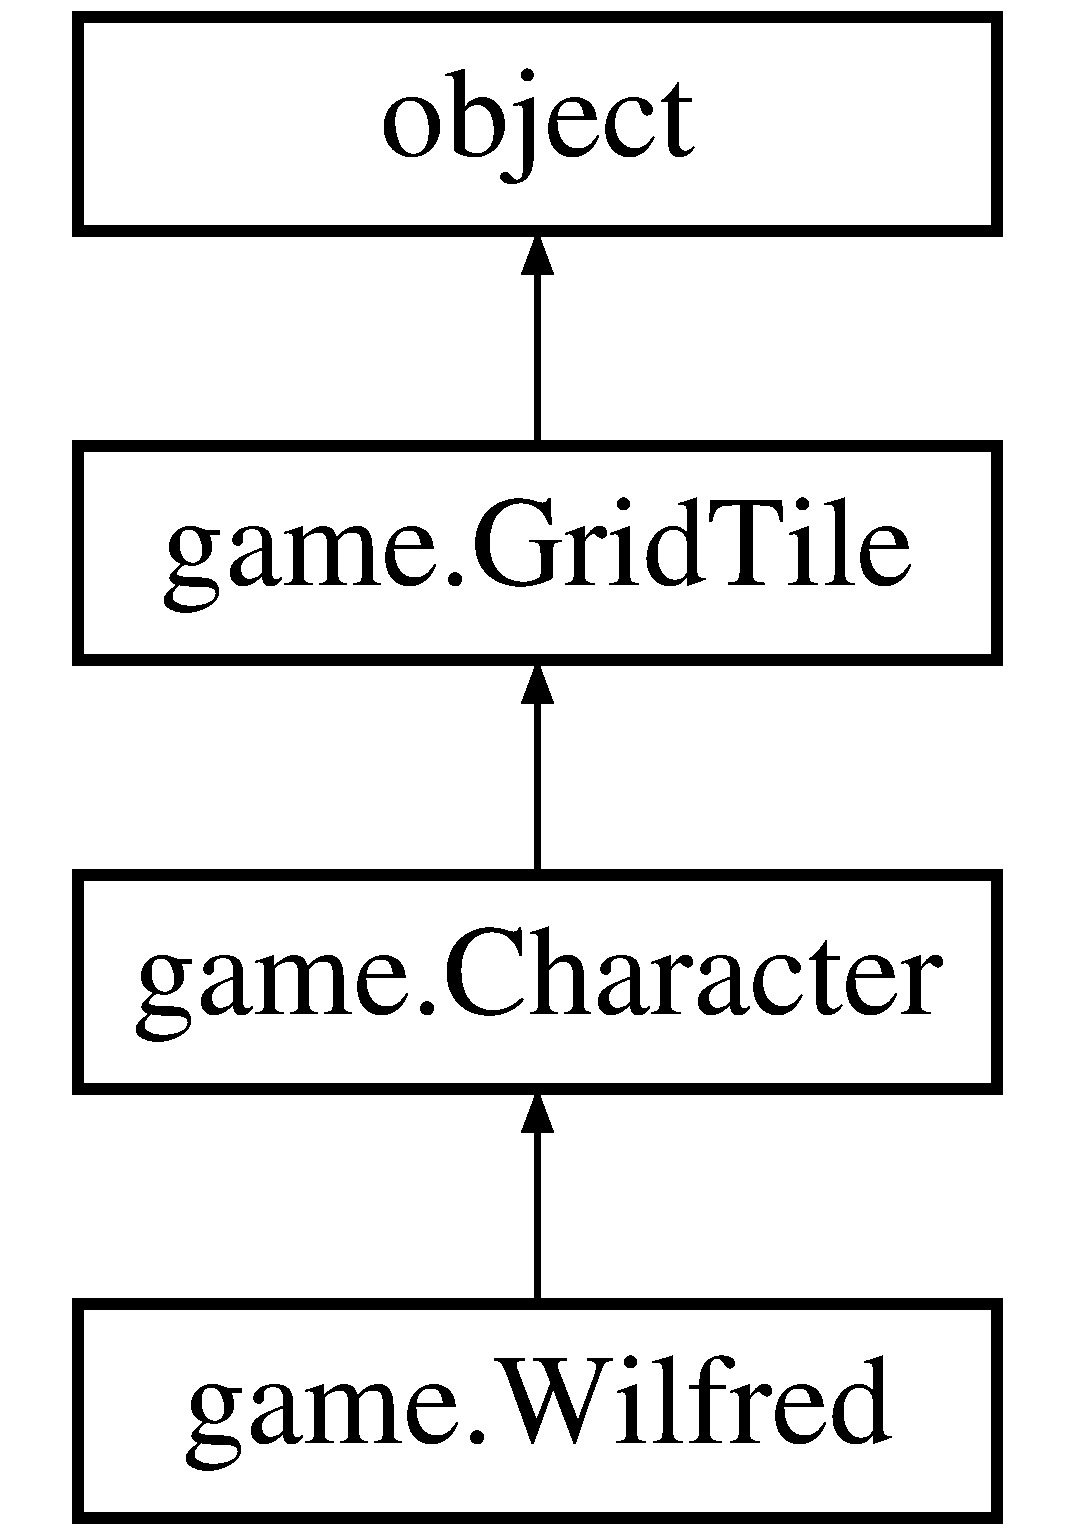
\includegraphics[height=4.000000cm]{classgame_1_1Wilfred}
\end{center}
\end{figure}
\subsection*{Public Member Functions}
\begin{DoxyCompactItemize}
\item 
\hypertarget{classgame_1_1Wilfred_ab07a2958da9b746ebb07d2f6515095a8}{def {\bfseries \-\_\-\-\_\-init\-\_\-\-\_\-}}\label{classgame_1_1Wilfred_ab07a2958da9b746ebb07d2f6515095a8}

\end{DoxyCompactItemize}
\subsection*{Public Attributes}
\begin{DoxyCompactItemize}
\item 
\hypertarget{classgame_1_1Wilfred_a8fc65d59b6ff8ed90856e78b19de2dbb}{{\bfseries image}}\label{classgame_1_1Wilfred_a8fc65d59b6ff8ed90856e78b19de2dbb}

\item 
\hypertarget{classgame_1_1Wilfred_a140998ca3f4800bb27f8b65a6a918c92}{{\bfseries move\-\_\-ability\-\_\-distance}}\label{classgame_1_1Wilfred_a140998ca3f4800bb27f8b65a6a918c92}

\item 
\hypertarget{classgame_1_1Wilfred_af85334a67807e86cece20cb929719b1f}{{\bfseries attack\-\_\-ability\-\_\-distance}}\label{classgame_1_1Wilfred_af85334a67807e86cece20cb929719b1f}

\item 
\hypertarget{classgame_1_1Wilfred_a904d6d5b9fae55d8b1f9f83f81d60907}{{\bfseries attack\-\_\-power}}\label{classgame_1_1Wilfred_a904d6d5b9fae55d8b1f9f83f81d60907}

\item 
\hypertarget{classgame_1_1Wilfred_a0e64de0f8001c025633fb20dec98bd70}{{\bfseries health\-\_\-points}}\label{classgame_1_1Wilfred_a0e64de0f8001c025633fb20dec98bd70}

\end{DoxyCompactItemize}


The documentation for this class was generated from the following file\-:\begin{DoxyCompactItemize}
\item 
game.\-py\end{DoxyCompactItemize}

%--- End generated contents ---

% Index
\newpage
\phantomsection
\addcontentsline{toc}{chapter}{Index}
\printindex

\end{document}
